\subsection{SCCs finden}
\begin{frame}{Wie findet man SCCs?}{}
\begin{wrapfigure}{r}{150px}
  \begin{center}
    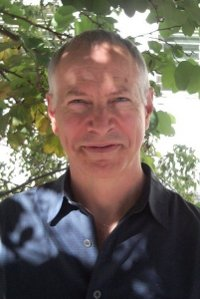
\includegraphics{Material/Bob_Tarjan.jpg}
  \end{center}
  \caption{Robert Tarjan}
\end{wrapfigure}
Algorithmus von Robert Tarjan

% Source: http://commons.wikimedia.org/wiki/File:Bob_Tarjan.jpg

nutzt Tiefensuche im Graphen
\end{frame}


\tikzstyle StackBox=[style=help lines,color=blue!50,fill=white]
\tikzstyle{abstract}=[rectangle, draw=black,
		fill=orange!40,
        text centered, anchor=center, text=white, text width=0.4cm, text height=0.4cm]
\tikzstyle{textstyle}=[rectangle, draw=white,
		fill=white, anchor=base west, text=black, text width=3cm, text height=0.4cm]
\tikzstyle{textstyleMini}=[rectangle, draw=white,
		fill=white, anchor=center, text=black, text width=0.5cm, text height=0.4cm]

\begin{frame}

\begin{algorithm}[H]
	\begin{algorithmic}
		\Function{startTarjan}{Graph g}
			\State $indexCounter \gets 0$
			\State $stack$
			\ForAll{$node$ in $g$}
				\If{$!node.visited$}
					\Call{tarjan}{$node$}
				\EndIf
			\EndFor
		\EndFunction
	\end{algorithmic}
\caption{Tarjans Algorithmus zur bestimmung starker Zusammenhangskomponenten}
\label{alg:seq1}
\end{algorithm}
\end{frame}

\begin{frame}
\begin{algorithm}[H]
    \begin{algorithmic}
        \Function{tarjan}{Node* node}
            \State $node.visited \gets $ \textbf{true}
            \State $node.index \gets indexCounter++$
            \State $stack.push(node)$
            \ForAll{$successor$ in $node.successors$}
                \If{$!node.visited$}
                    \Call{tarjan}{successor}
                \EndIf
                \State $node.lowlink \gets$ \Call{min}{$node.lowlink, successor.lowlink$}
            \EndFor

            \boxto<1->{a}\If{$node.lowlink == node.index$}
                \Repeat
                    \State $successor \gets stack.pop()$
                \Until{$successor == node$}
            \EndIf\tikzmark{a}
        \EndFunction
    \end{algorithmic}
\label{alg:seq2}
\end{algorithm}

% To insert the annotation
\begin{tikzpicture}[remember picture,overlay]
\coordinate (a) at ($(a)+(8.5,3)$); % <= adjust this parameter to move the position of the annotation
\node[rectangle,draw, gray,text width=3cm,align=left,right] at (a) {SCC wurde gefunden, ggf. ausgeben};
\end{tikzpicture}
\end{frame}

\begin{frame}{Wie findet man SCCs?}{}
	\begin{figure}
		\begin{tikzpicture}[->,scale=1.8, auto,swap]
			\node[textstyle] (Text) at (0,3) {Rekursionstiefe:};
			\node[textstyle] (RecDepth) at (3,3) {};

			% Draw the vertices
			\foreach \pos/\name in {{(0,0)/a}, {(0,2)/b}, {(1,2)/c},
				                    {(1,0)/d}, {(2,1)/e}, {(3,1)/f},
									{(4,2)/g}, {(5,2)/h}, {(4,0)/i},
									{(5,0)/j}}
				\node[vertex] (\name) at \pos {$\name$};

			% Connect vertices with edges
			\foreach \source/ \dest /\pos in {a/b/,b/c/,c/d/,d/a/,
										c/e/bend left, d/e/,e/c/,
										e/f/,
										f/g/, f/i/,g/f/bend right,i/f/bend left,
										g/h/, h/j/, j/i/, i/g/}
				\path (\source) edge [\pos] node {} (\dest);

			% Start animating the vertex and edge selection.
			\foreach \vertex / \fr / \lowlink / \index in {a/1/0/0,b/2/1/1,c/3/2/2,d/4/0/3,e/5/2/4,f/6/5/5,g/7/6/6,h/8/7/7,j/9/8/8,i/10/5/9} {
				\path<\fr-> node[selected vertex] at (\vertex) {$\vertex_{\lowlink, \index}$};
				\path<\fr-> node[textstyleMini] at (RecDepth) {$\index$};
			}
			% Start animating the edge selection.
			% For convenience we use a background layer to highlight edges
			% This way we don't have to worry about the highlighting covering
			% weight labels.
			\begin{pgfonlayer}{background}
				    \path<4->[ignored edge] (d.center) edge [] node {} (a.center);
				    \path<5->[ignored edge] (e.center) edge [] node {} (c.center);
				    \path<10->[ignored edge] (i.center) edge [bend left] node {} (f.center);
				\foreach \source / \dest / \fr / \pos in {a/b/2/,b/c/3/,c/d/4/, d/e/5/,e/f/6/,f/g/7/,g/h/8/,
														h/j/9/,j/i/10/}
				    \path<\fr->[selected edge] (\source.center) edge [\pos] node {} (\dest.center);
			\end{pgfonlayer}
			% go back in recursion
			% Start animating.
			\foreach \vertex / \fr / \lowlink / \index in {j/11/5/8,h/12/5/7,g/13/5/6,f/14/5/5} {
				\path<\fr-> node[selected vertex] at (\vertex) {$\vertex_{\lowlink, \index}$};
				\path<\fr-> node[textstyleMini] at (RecDepth) {$\index$};
			}
			% mark first scc
			\begin{pgfonlayer}{background}
				\path<15->[color=blue,fill=green!20] (4.2,1) circle (1.6cm);
			\end{pgfonlayer}
			% go back in recursion
			% Start animating.
			\foreach \vertex / \fr / \lowlink / \index in {e/16/2/4,c/17/0/3,b/18/0/1,a/19/0/0} {
				\path<\fr-> node[selected vertex] at (\vertex) {$\vertex_{\lowlink, \index}$};
				\path<\fr-> node[textstyleMini] at (RecDepth) {$\index$};
			}
			% mark first scc
			\begin{pgfonlayer}{background}
				\path<20->[color=blue,fill=green!20] (0.6,1) circle (1.6cm);
			\end{pgfonlayer}
		\end{tikzpicture}
	\end{figure}
\end{frame}
